%%%%%%%%%%%%%%%%%%%%%%%%%%%%%%%%%%%%%%%%%%%%%%%%%%%
%% LaTeX book template                           %%
%% Author:  Amber Jain (http://amberj.devio.us/) %%
%% License: ISC license                          %%
%%%%%%%%%%%%%%%%%%%%%%%%%%%%%%%%%%%%%%%%%%%%%%%%%%%

\documentclass[a4paper,11pt]{book}

\usepackage[T1]{fontenc}
\usepackage[utf8]{inputenc}
\usepackage{lmodern}
\usepackage{hyperref}
\usepackage{graphicx}
\usepackage[portuguese]{babel}
\usepackage{amsfonts}
\usepackage[usenames,dvipsnames]{xcolor}

% para usar definições
\usepackage{amsthm}

\theoremstyle{definition}
\newtheorem{definition}{Definition}[section]

% tirando identação dos paragrafos
\setlength{\parindent}{0ex}

% coding examples in latex file
\usepackage{listings}
\usepackage{xcolor}

\definecolor{codegreen}{rgb}{0,0.6,0}
\definecolor{codegray}{rgb}{0.5,0.5,0.5}
\definecolor{codepurple}{rgb}{0.58,0,0.82}
\definecolor{backcolour}{rgb}{0.95,0.95,0.92}

\lstdefinestyle{mystyle}{
    backgroundcolor=\color{backcolour},   
    commentstyle=\color{codegreen},
    keywordstyle=\color{magenta},
    numberstyle=\tiny\color{codegray},
    stringstyle=\color{codepurple},
    basicstyle=\ttfamily\footnotesize,
    breakatwhitespace=false,         
    breaklines=true,                 
    captionpos=b,                    
    keepspaces=true,                 
    numbers=left,                    
    numbersep=5pt,                  
    showspaces=false,                
    showstringspaces=false,
    showtabs=false,                  
    tabsize=2
}

\lstset{style=mystyle}

%%%%%%%%%%%%%%%%%%%%%%%%%%%%%%%%%%%%%%%%%%%%%%%%%%%%%%%%%%%%%%%%%%%%%%%%%%%%%%%%
% 'dedication' environment: To add a dedication paragraph at the start of book %
% Source: http://www.tug.org/pipermail/texhax/2010-June/015184.html            %
%%%%%%%%%%%%%%%%%%%%%%%%%%%%%%%%%%%%%%%%%%%%%%%%%%%%%%%%%%%%%%%%%%%%%%%%%%%%%%%%
\newenvironment{dedication}
{
   \cleardoublepage
   \thispagestyle{empty}
   \vspace*{\stretch{1}}
   \hfill\begin{minipage}[t]{0.66\textwidth}
   \raggedright
}
{
   \end{minipage}
   \vspace*{\stretch{3}}
   \clearpage
}

%%%%%%%%%%%%%%%%%%%%%%%%%%%%%%%%%%%%%%%%%%%%%%%%
% Chapter quote at the start of chapter        %
% Source: http://tex.stackexchange.com/a/53380 %
%%%%%%%%%%%%%%%%%%%%%%%%%%%%%%%%%%%%%%%%%%%%%%%%
\makeatletter
\renewcommand{\@chapapp}{}% Not necessary...
\newenvironment{chapquote}[2][2em]
  {\setlength{\@tempdima}{#1}%
   \def\chapquote@author{#2}%
   \parshape 1 \@tempdima \dimexpr\textwidth-2\@tempdima\relax%
   \itshape}
  {\par\normalfont\hfill--\ \chapquote@author\hspace*{\@tempdima}\par\bigskip}
\makeatother


%%%%%%%%%%%%%%%%%%%%%%%%%%%%%%%%%%%%%%%%%%%%%%%%%%%
% First page of book which contains 'stuff' like: %
%  - Book title, subtitle                         %
%  - Book author name                             %
%%%%%%%%%%%%%%%%%%%%%%%%%%%%%%%%%%%%%%%%%%%%%%%%%%%
% Book's title and subtitle
\title{\Huge \textbf{Book of Proof} \\ 
\huge Third Edition}
% Author
\author{\textsc{Richard Hammack}}


\begin{document}

\frontmatter
\maketitle

\tableofcontents
%\listoffigures
%\listoftables

\mainmatter

%%%%%%%%%%%%%%%%%%%%%%%%%%%%%%%%%%%%%%%%%%%%%%%%%%%
%                 CHAPTER                         %
%%%%%%%%%%%%%%%%%%%%%%%%%%%%%%%%%%%%%%%%%%%%%%%%%%%
\chapter{Conjuntos}


\begin{chapquote}{página 3}
	``The theory of sets is a language that is perfectly suited to describing and explaning all types of mathematical structures.''
\end{chapquote}


\section{Introdução}
Um \textbf{conjunto} (set) é uma lista de \textbf{elementos}. Normalmente denotados por uma letra maiúscula. Por exemplo:

\begin{center}
	$ A = \{1 , 2 , 3 , 4 , ... \} $
\end{center}

Dois sets $A$ e $B$ são \textbf{iguais} se possuírem exatamente os mesmos elementos. Não importando a ordem desses elementos dentro de cada set.
\\
\\
Vamos definir um símbolo para sinalizar se um determinado elemento $x$ pertence ou não a um determinado set qualquer $A$. Para tal relação usaremos o símbolo $"\in"$ se $x$ for um elemento de $A$ ou, caso contrário, usaremos $"\notin"$ se $x$ não for um elemento de $A$.
\\
\\
É provável que, em algum momento, seja necessário contar a quantidade de elementos em um dado set qualquer $A$. Chamaremos essa relação de \textbf{cardinalidade} ou \textbf{tamanho} do set $A$. O símbolo usado será duas barras em volta do set do seguinte modo: "$|A|$".
\\
\\
A partir dessas duas relações já podemos definir um tipo especial de set. Vamos definir como \textbf{conjunto vazio} ou \textbf{empty set} um conjunto que possua o cardinal igual a zero. Usaremos o símbolo $"\emptyset"$ para definir a relação abaixo:

\begin{center}
	$|\emptyset| = 0$
\end{center}

Às vezes, não raramente, usamos sets que a escrita como uma lista de elementos não é tão intuitiva para uso. Para essas situações usamos a \textbf{notação de formação de conjuntos (set builder notation)}. Como no exemplo abaixo:

\begin{center}
	$ E = $ \textcolor{red}{$\{$} \textcolor{blue}{$2n$} \textcolor{OliveGreen}{$:$} \textcolor{Brown}{$n$} \textcolor{Orange}{$\in$} $\mathbb{Z} \}$
\end{center}

Eu colori cada significado da expressão acima com a cor correspondente para facilitar o entendimento. A leitura da expressão acima é: "O conjunto '$E$' é igual ao \textcolor{red}{conjunto dos elementos da forma} \textcolor{blue}{$2n$} \textcolor{OliveGreen}{tal que} \textcolor{Brown}{$n$} \textcolor{Orange}{é um elemento de} $\mathbb{Z}$".
\\
\\
Podemos resumir essa notação de formação de conjuntos como "$Conjunto = \{ Expressão : Regra \}$". É bem comum vermos notações onde os dois pontos são trocados por uma barra: "$Conjunto = \{ Expressão \ | \ Regra \}$".
\\
\\
Existem alguns conjuntos que são famosos e a essa altura você já deve ter visto algumas vezes.
\begin{itemize}
	\item[] $\emptyset = \{ \}$
	\item[] $\mathbb{N} = \{ 1, 2, 3, 4, ... \}$, perceba que $0 \notin \mathbb{N}$
	\item[] $\mathbb{Z} = \{ ..., -2, -1, 0, 1, 2, ...  \}$
	\item[] $\mathbb{Q} = \{ x : x = m/n, \ onde \ m,n \in \mathbb{Z} \  e \  n \neq 0 \}$
	\item[] 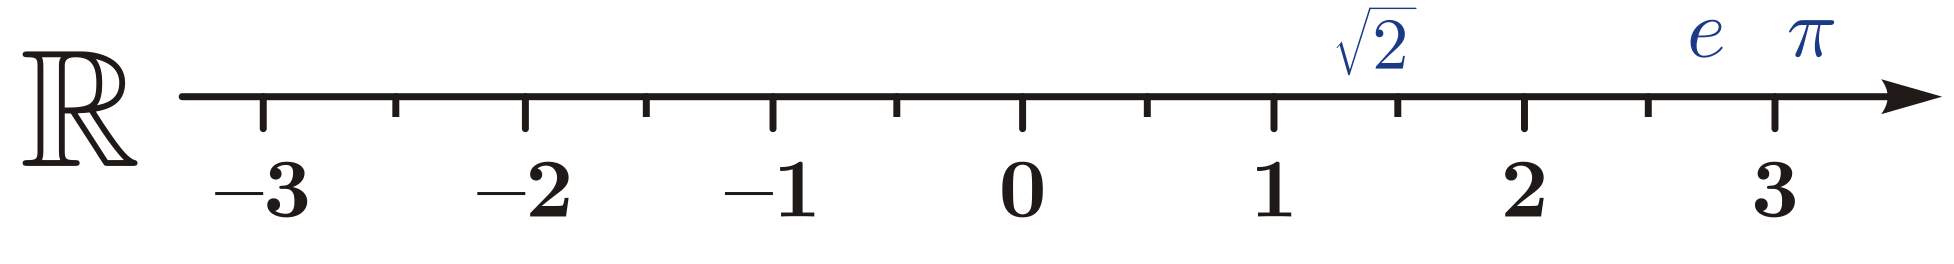
\includegraphics[scale=0.11]{images/real_line.png}
\end{itemize}

Como o conjunto dos número reais pode ser descrito como pontos em uma reta infinita. Se tivermos dois pontos quaisquer $a$ e $b$, de modo que, $a,b \in \mathbb{R}$ e $a < b$. Temos infinitos elementos entre esses dois pontos. Desse modo, teremos que usar um novo símbolo para se referir aos conjuntos que são melhor descritos em termos de \textbf{intervalos} entre pontos.
\begin{center}
	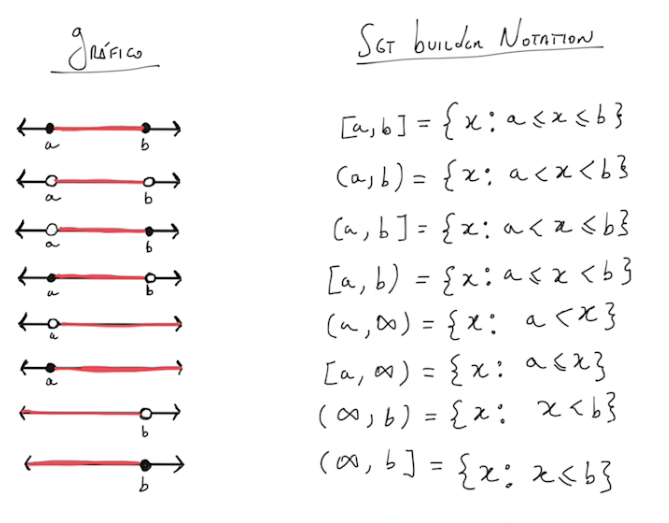
\includegraphics[scale=0.7]{images/intervals.png}
\end{center}

\section{Produto Cartesiano}
\begin{definition}[Par Ordenado]
Um \textbf{par ordenado} é um lista na forma $(x, y)$ que contém dois elementos ($x$ e $y$). Onde esses dois elementos estão entre parênteses e separados por uma vírgula.
\end{definition}

Atente para o fato que $(x,y) \neq (y,x)$. 
\\
\\
Agora que temos a definição de par ordenado. Podemos escrever conjuntos usando esse novo símbolo.

\begin{definition}[Produto Cartesiano]
O \textbf{produto cartesiano} de dois sets $A$ e $B$ é um outro set cujo símbolo é $``A \times B"$ e é definido como:
\begin{center}
$A \times B = \{ (a,b) : a \in A, b \in B \}$
\end{center}
\end{definition}

Perceba que, se $A$ e $B$ são finitos, então $| A \times B | = |A| . |B|$
%%%%%%%%%%%%%%%%%%%%%%%%%%%%%%%%%%%%%%%%%%%%%%%%%%%
%                 CHAPTER                         %
%%%%%%%%%%%%%%%%%%%%%%%%%%%%%%%%%%%%%%%%%%%%%%%%%%%
\chapter{Lógica}


%%%%%%%%%%%%%%%%%%%%%%%%%%%%%%%%%%%%%%%%%%%%%%%%%%%
%                 CHAPTER                         %
%%%%%%%%%%%%%%%%%%%%%%%%%%%%%%%%%%%%%%%%%%%%%%%%%%%
\chapter{Contagem}
\chapter{Prova Direta}
\chapter{Prova Contra-positiva}
\chapter{Prova por Contradição}
\chapter{Prova de Afirmações Não-Condicionais}
\chapter{Provas Envolvendo Conjuntos}
\chapter{Contraprova}
\chapter{Indução Matemática}
\chapter{Relações}
\chapter{Funções}
\chapter{Provas com Calculus}
\chapter{Cardinalidade de Conjuntos}

\end{document}